\chapter{Zentralspinmodell}

\begin{wrapfigure}{r}{0.4\textwidth}
    \centering
    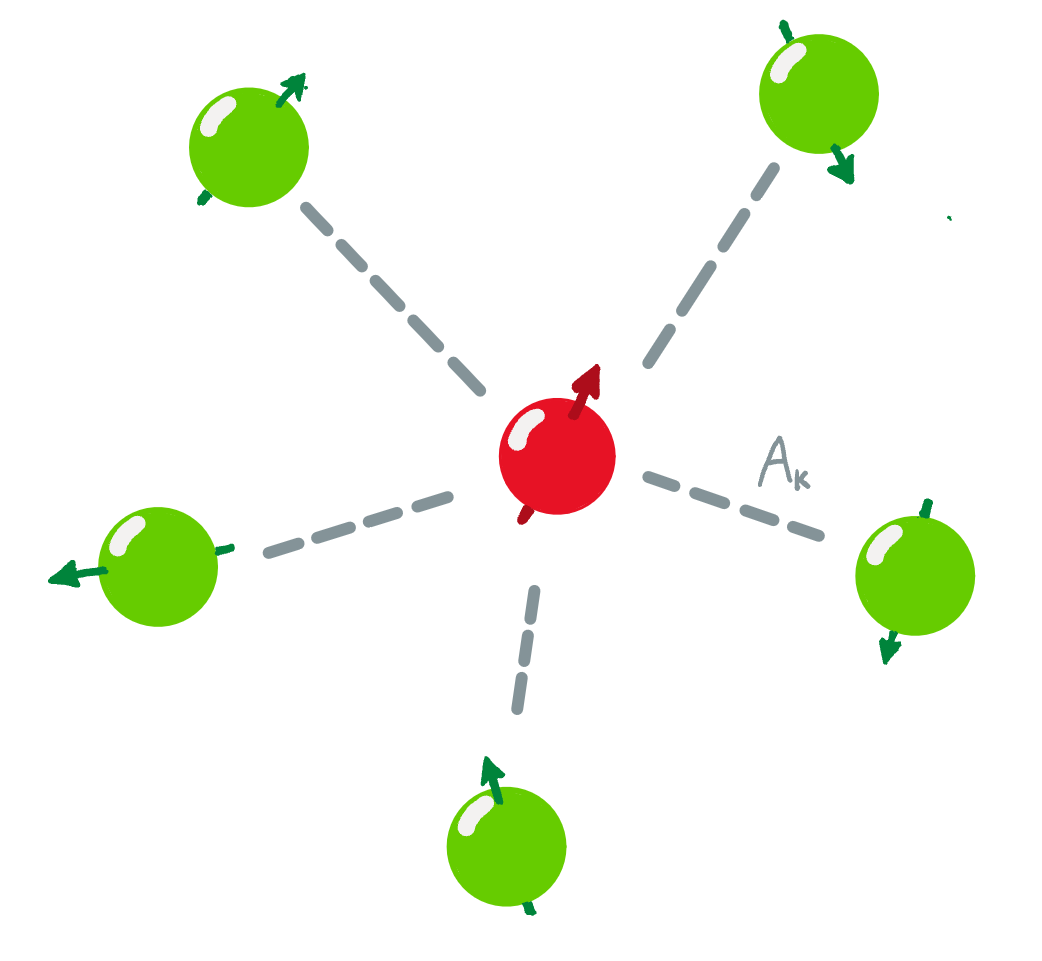
\includegraphics[width = 0.35\textwidth]{Abbildungen/CSM_Schema_Salem.png}
    \caption{Schematischer Aufbau des Zentralspinmodell mit dem Elektronenspins (Rot) und den in direkter Umgebung liegenden 
    Kernspins (Grün) und einer Kopplungskonstante $A_k$}
    \label{fig:CSM}
\end{wrapfigure}
%CSM: https://iopscience.iop.org/article/10.1088/1367-2630/16/6/065023
Im folgenden wird das \textbf{Zentralspinmodell} zur Beschreibung der Spindynamik des Quantenpunktes verwendet. Dabei werden die Interaktionen des 
Elektronenspins mit dem externen Magnetfeld $\vec{B}$ und den umliegenden Kernspins $\hat{\vec{I}}_k$ über eine Heisenbergkopplung $A_k$ berücksichtigt.
Die Kernspins wechselwirken dabei auch mit dem äußeren Magnetfeld, aber die Wechselwirkung untereinander wird vernachlässigt.
\begin{align}
    \overline{\hat{H}}_{CSM} &= \mu_B\thinspace g_e \vec{B}\hat{\vec{S}} +  \sum_{k=1}^{N}\mu_k\thinspace g_k\vec{B}\hat{\vec{I}}_k + \sum_{k=1}^{N} A_k \hat{\vec{S}}\hat{\vec{I}}_k
\end{align}
Dabei entspricht anders als beim freien Elektron der g-Faktor eines Elektron im Quantenpunkt nicht mehr 2, sondern ca. 0,555. \cite{PMID:17901328}
Das Kernmagneton $\mu_k= 5,05 \cdot 10^{27} \frac{J}{T}$ ist etwa 1800 Mal kleiner als das Bohrsche 
Magneton $\mu_B = 9.27 \cdot 10^{24} \frac{J}{T}$\cite{Dyakonov2008-ub}. Die g-Faktoren $g_k$ können für alle Kernspins der 
Einfachheit halber als gleich angenommen werden. \\
Im folgenden wird die charakteristische Zeitskala $T^*$ wird verwendet, welcher den Einfluss der führenden Ordnung des Materials,
mit der ein einzelnes Elektron in eine 
, that describes the
leading order impact of the material, which forms the confinement potential to trap a
single electron or hole, on the central spin dynamics 
\begin{align}
    T^* &= \frac{1}{\sqrt{\sum_k A_k^2\langle \hat{I}_k^2 \rangle}}
\end{align}
Nun kann der dimensionslose Hamiltonian $\hat{H}_{CSM} = T^*\thinspace\overline{\hat{H}}_{CSM}$ hingeschrieben werden:
\begin{align}
    \hat{H}_{CSM} &= \vec{b}\hat{\vec{S}} +  \sum_{k=1}^{N}z_k\vec{b}\hat{\vec{I}}_k + \sum_{k=1}^{N} \alpha_k \hat{\vec{S}}\hat{\vec{I}}_k
\end{align}
% \langle\Psi(t) \mid \dot{\Psi}(t)\rangle
mit $\vec{b}=T^*\mu_B\thinspace g_e \vec{B}$ , der Zeeman-Konstante $z_k=T^*\frac{\mu_I g_k}{\mu_B g_e}$ und $\alpha_k = T^* A_k$.


